\chapter{Checklist}
\label{cp:checklist}
Following is the comprehensive checklist\footnote{Starting from this page,for each species; \textbf{H:}, \textbf{D:}, \textbf{R:} indicates \textit{"Habitat \& distribution in Sri Lanka"}, \textit{"Diet"} and \textit{"Recorded areas inside the university"} respectively.} of bird species recorded in the university premises of University of Moratuwa according to the collected data of sightings from 2021 to 2024 (with their respective conservation statuses[3]).

\begin{itemize}%
\item%
 Accipitridae%
\begin{enumerate}%
\item%
\begin{description}%
\item[]%
\textit{Haliastur indus (LC)}%
\item[]%
\textbf{Brahminy Kite}%
\end{description}%
\begin{description}%
\item[H: ]%
Very common breeding resident in lowlands. Regular but rare visitor to the hills. Can be observed easily near water mainly in coastal areas and large inland wetlands and also along rivers{[}2{]}.%
\item[D: ]%
Fish, snakes, lizards, frogs, and small mammals. They soar high in the air and swoop down to catch their prey.%
\item[R: ]%
Most commonly observed during flight throughout the university. Perched specimen can be spotted near the university ground premises and the bolgoda lakeside trees.%
\end{description}%
\item%
\begin{description}%
\item[]%
\textit{Accipiter badius (LC)}%
\item[]%
\textbf{Shikra}%
\end{description}%
\begin{description}%
\item[H: ]%
Common breeding resident throughout the entire island. Can be observed in both open country and in dense forest. Specially can be observed in close proximity with residential areas too{[}2{]}.%
\item[D: ]%
 Lizards, birds, snakes, and insects. They hunt from perches or by flying low over the ground.%
\item[R: ]%
Perched on trees around the ground and in Kaju Kele and in flight at Boat yard area.%
\end{description}%
\item%
\begin{description}%
\item[]%
\textit{Pernis ptilorhynchus (VU)}%
\item[]%
\textbf{Oriental Honey-buzzard}%
\end{description}%
\begin{description}%
\item[H: ]%
Fairly rare breeding resident and the population much increased by the winter migrants. Occurs throughout the island. Mostly observed in well{-}wooded areas{[}2{]}.%
\item[D: ]%
Primarily larvae, pupae, and honeycombs of social wasps and bees, occasionally supplemented with cicadas, small birds, reptiles, and frogs.%
\item[R: ]%
Edges of the university ground, boat yard and the surrounding trees.%
\end{description}%
\item%
\begin{description}%
\item[]%
\textit{Haliaeetus leucogaster (LC)}%
\item[]%
\textbf{White{-}bellied Sea Eagle}%
\end{description}%
\begin{description}%
\item[H: ]%
Kind of uncommon breeding resident in lowlands and up to lower hills, more common in dry lowlands and regular visitor to higher hills. Mainly observed in near vicinity of coasts, large tanks and also along rivers{[}2{]}.%
\item[D: ]%
Primarily fish, scavenged carrion, and occasionally reptiles and crustaceans. They hunt by soaring and diving, snatching prey from the water's surface.%
\item[R: ]%
Around the university ground and the boat yard area.%
\end{description}%
\item%
\begin{description}%
\item[]%
\textit{Nisaetus cirrhatus (LC)}%
\item[]%
\textbf{Changeable Hawk{-}Eagle/Crested Hawk{-}Eagle}%
\end{description}%
\begin{description}%
\item[H: ]%
Fairly common locally throughout the island and a breeding resident. Well wooded areas is the preferred habitat{[}2{]}.%
\item[D: ]%
Has a diverse diet, preying on a variety of animals including mammals, large birds, reptiles such as snakes and lizards, fish and amphibians like frogs.%
\item[R: ]%
Observed only once in the boat yard at the opposite bank.%
\end{description}%
\end{enumerate}%
\item%
Alcedinidae%
\begin{enumerate}%
\item%
\begin{description}%
\item[]%
\textit{Pelargopsis capensis (LC)}%
\item[]%
\textbf{Stork{-}billed Kingfisher}%
\end{description}%
\begin{description}%
\item[H: ]%
Uncommon breeding resident from lowlands up to lower hills. Wooded banks of rivers and streams, lakes and paddy-fields adjoining wooded areas, tanks, lagoons and mangrove edged creeks are the habitat where mostly can be seen.{[}2{]}.%
\item[D: ]%
Mainly consists of fresh water fish species, crustaceans, frogs and sometimes small rodents.%
\item[R: ]%
Boat yard and the surrounding areas of Bolgoda lake.%
\end{description}%
\item%
\begin{description}%
\item[]%
\textit{Halcyon smyrnensis (LC)}%
\item[]%
\textbf{White{-}breasted Kingfisher/White{-}throated Kingfisher}%
\end{description}%
\begin{description}%
\item[H: ]%
Common breeding resident found throughout the island. Can be observed in open areas, cultivation, gardens and wetlands. The most common Kingfisher species in Sri Lanka{[}2{]}.%
\item[D: ]%
Has a diverse range of prey, including large crustaceans, insects, earthworms, rodents, lizards, snakes, fish, and frogs. Occasionally preys on small birds.%
\item[R: ]%
Near the university playground, hostels and fairly common in boat yard and Kaju Kele.%
\end{description}%
\item%
\begin{description}%
\item[]%
\textit{Ceryle rudis (LC)}%
\item[]%
\textbf{Pied Kingfisher}%
\end{description}%
\begin{description}%
\item[H: ]%
Fairly uncommon breeding resident in lowlands. occasionally visits low hills. Paddy-fields,streams,tanks and coastal areas of estuaries,lagoons,large tanks and slow moving rivers are the preferred habitat{[}2{]}.%
\item[D: ]%
The primary diet of this species comprises fish. Occasionally consumes crustaceans and large aquatic insects such as dragonfly larvae.%
\item[R: ]%
Boat yard and the surrounding areas of Bolgoda lake.%
\end{description}%
\item%
\begin{description}%
\item[]%
\textit{Alcedo atthis (LC)}%
\item[]%
\textbf{Common Kingfisher}%
\end{description}%
\begin{description}%
\item[H: ]%
Somewhat uncommon breeding resident throughout Sri Lanka, but rare in higher hills. Wetlands, open country and forests are the preferred habitat{[}2{]}.%
\item[D: ]%
Primary diet consists mainly of small fish, although it also includes insect larvae and, occasionally frogs.%
\item[R: ]%
Boat yard and the surrounding areas of Bolgoda lake.%
\end{description}%
\end{enumerate}%
\item%
Anatidae%
\begin{enumerate}%
\item%
\begin{description}%
\item[]%
\textit{Dendrocygna javanica (LC)}%
\item[]%
\textbf{Lesser Whistling{-}Duck}%
\end{description}%
\begin{description}%
\item[H: ]%
Common breeding resident throughout the lowlands. Migrant population also has been identified during the northern winter season. Can be commonly observed in fresh water marshes and tanks{[}2{]}.%
\item[D: ]%
Mainly on plants taken from the water as well as grains from cultivated rice apart from small fish, frogs and invertebrates such as molluscs and worms%
\item[R: ]%
Boat yard and the surrounding areas of Bolgoda lake.%
\end{description}%
\end{enumerate}%
\item%
Anhingidae%
\begin{enumerate}%
\item%
\begin{description}%
\item[]%
\textit{Anhinga melanogaster (LC)}%
\item[]%
\textbf{Oriental Darter}%
\end{description}%
\begin{description}%
\item[H: ]%
Uncommon breeding resident in dry lowlands. Very rarely observed in wet lowlands and high hills. Tanks, lakes, larger rivers and lagoons are the preferred habitat{[}2{]}.%
\item[D: ]%
Mainly fish, particularly snakeheads and mudfish.%
\item[R: ]%
Boat yard and the surrounding areas of Bolgoda lake.%
\end{description}%
\end{enumerate}%
\item%
Apodidae%
\begin{enumerate}%
\item%
\begin{description}%
\item[]%
\textit{Cypsiurus balasiensis (LC)}%
\item[]%
\textbf{Asian Palm Swift}%
\end{description}%
\begin{description}%
\item[H: ]%
Common breeding resident throughout Sri Lanka. Mainly observed around fan palms{[}2{]}.%
\item[D: ]%
Primarily sustains itself on an insect{-}based diet such as grasshoppers, moths, crickets, mantises, beetles, dragonflies and flying termites.%
\item[R: ]%
Surrounding woody areas of the university playground and open banks of Bolgoda lake near boat yard.%
\end{description}%
\item%
\begin{description}%
\item[]%
\textit{Aerodramus unicolor (VU)}%
\item[]%
\textbf{Indian Swiftlet}%
\end{description}%
\begin{description}%
\item[H: ]%
Common breeding resident found throughout Sri Lanka. Roosts and breeds inside cav{[}2{]}.%
\item[D: ]%
Diet comprises a variety of insects, including flies, wasps, bees, cicadas, flying termites, beetles, grasshoppers, airborne spiders, and butterflies.%
\item[R: ]%
Surrounding woody areas of the university playground.%
\end{description}%
\end{enumerate}%
\item%
Ardeidae%
\begin{enumerate}%
\item%
\begin{description}%
\item[]%
\textit{Ardea intermedia (LC)}%
\item[]%
\textbf{Intermediate Egret/Medium Egret}%
\end{description}%
\begin{description}%
\item[H: ]%
Uncommon breeding resident found from lowlands to hills. Commonly observed in marshes, paddy-fields and shallow vegetated edges of tanks and lagoons{[}2{]}.%
\item[D: ]%
Fish, frogs, insects, and crustaceans. They forage in shallow water, often stalking their prey.%
\item[R: ]%
Boat yard and the surrounding areas of Bolgoda lake.%
\end{description}%
\item%
\begin{description}%
\item[]%
\textit{Ardea purpurea (LC)}%
\item[]%
\textbf{Purple Heron}%
\end{description}%
\begin{description}%
\item[H: ]%
Common breeding resident in lowlands and ascends up to lower hills, but rare in hills.Can be spotted in vegetation of marshes, paddy-fields and tanks.{[}2{]}.%
\item[D: ]%
Fish, frogs, insects, and small mammals.%
\item[R: ]%
Boat yard and the surrounding areas of Bolgoda lake.%
\end{description}%
\item%
\begin{description}%
\item[]%
\textit{Ardeola grayii (LC)}%
\item[]%
\textbf{Indian Pond{-}Heron}%
\end{description}%
\begin{description}%
\item[H: ]%
 Common breeding residents that can be found all throughout Sri Lanka and numerous winter migrants appear to arrive all over the country{[}2{]}.%
\item[D: ]%
Consists of crustaceans, aquatic insects, fishes, tadpoles and sometimes leeches. Outside wetlands, these herons regularly feed on insects.%
\item[R: ]%
Boat yard and the surrounding areas of Bolgoda lake.%
\end{description}%
\item%
\begin{description}%
\item[]%
\textit{Nycticorax nycticorax (LC)}%
\item[]%
\textbf{Black{-}crowned Night{-}Heron}%
\end{description}%
\begin{description}%
\item[H: ]%
Common breeding resident throughout the lowlands  up to lower hills. Occasionally ascends to higher hills too. Can be observed in marshes, mangroves and other vegetation at edge of rivers,tanks and lagoons as well as tree covered islands{[}2{]}.%
\item[D: ]%
Fish, frogs, crabs, and insects. They are nocturnal hunters and forage in wetlands and rice paddies.%
\item[R: ]%
Boat yard and the surrounding areas of Bolgoda lake.%
\end{description}%
\item%
\begin{description}%
\item[]%
\textit{Ardea cinerea (LC)}%
\item[]%
\textbf{Grey Heron}%
\end{description}%
\begin{description}%
\item[H: ]%
Fairly common breeding resident in dry lowlands. Rare in wet lowlands. Occasional records are present at high hills up to 2000m. Coastal lagoons, marshes, and tanks are the preferred habitats{[}2{]}.%
\item[D: ]%
Main diet consists of fish. May also consume amphibians, crustaceans, snakes, small birds, rodents, and occasionally, certain plants.%
\item[R: ]%
Boat yard and the surrounding areas of Bolgoda lake. Mostly observed in flight.%
\end{description}%
\item%
\begin{description}%
\item[]%
\textit{Butorides striata (LC)}%
\item[]%
\textbf{Striated Heron}%
\end{description}%
\begin{description}%
\item[H: ]%
Fairly uncommon breeding resident in lowlands and lower hills. Mangroves and dense vegetation at the edges of the rivers, marshes and tanks, open edges of lagoons are the preferred habitats{[}2{]}.%
\item[D: ]%
Primarily feeds on a diet consisting of crabs and other crustaceans. Additionally, it includes mollusks and small fish in its feeding repertoire.%
\item[R: ]%
Can be observed at Boat yard mostly in flight.%
\end{description}%
\item%
\begin{description}%
\item[]%
\textit{Bubulcus ibis (LC)}%
\item[]%
\textbf{Cattle Egret/Eastern Cattle Egret}%
\end{description}%
\begin{description}%
\item[H: ]%
Common migratory bird and can be seen throughout the country. Often seen around herds of cattle{[}2{]}.%
\item[D: ]%
Primary diet consists of large insects such as grasshoppers, crickets, and flies. They may also include frogs, spiders, moths in their diet.%
\item[R: ]%
University playground premises and the Boat yard.%
\end{description}%
\item%
\begin{description}%
\item[]%
\textit{Egretta garzetta (LC)}%
\item[]%
\textbf{Little Egret}%
\end{description}%
\begin{description}%
\item[H: ]%
Fairly common breeding resident from lower hills to lowlands. Uncommon in high hills{[}2{]}.%
\item[D: ]%
They primarily consume fish, although their diet also includes amphibians, small reptiles, mammals, and small birds.%
\item[R: ]%
Boat yard and the surrounding areas of Bolgoda lake.%
\end{description}%
\end{enumerate}%
\item%
Campephagidae%
\begin{enumerate}%
\item%
\begin{description}%
\item[]%
\textit{Pericrocotus cinnamomeus (LC)}%
\item[]%
\textbf{Small Minivet}%
\end{description}%
\begin{description}%
\item[H: ]%
Uncommon breeding resident from lowlands up to mid hills. Open forests and bushes with scattered trees are the places to look for{[}2{]}.%
\item[D: ]%
Primarily feed on an insect{-}based diet, which includes caterpillars, beetles, bugs, and ants.%
\item[R: ]%
Observed in the tree canopy of Kaju Kele and behind the building located in Boat yard.%
\end{description}%
\end{enumerate}%
\item%
Charadriidae%
\begin{enumerate}%
\item%
\begin{description}%
\item[]%
\textit{Vanellus indicus (LC)}%
\item[]%
\textbf{Red{-}wattled Lapwing}%
\end{description}%
\begin{description}%
\item[H: ]%
Common breeding resident throughout the island but somewhat rare in hills. Can be commonly in open flat grounds located in the near vicinity of water{[}2{]}.%
\item[D: ]%
Insects, worms, and other invertebrates. They forage by running and probing the ground with their long bills.%
\item[R: ]%
Observed very commonly in the university ground premises.%
\end{description}%
\end{enumerate}%
\item%
Chloropseidae%
\begin{enumerate}%
\item%
\begin{description}%
\item[]%
\textit{Chloropsis jerdoni (LC)}%
\item[]%
\textbf{Jerdon's Leafbird}%
\end{description}%
\begin{description}%
\item[H: ]%
Uncommon breeding resident from lowlands up to mid hills. More common to see in dry zone. Forests, wooded areas and gardens are the preferred habitats{[}2{]}.%
\item[D: ]%
This species feeds on eats insects, fruit and nectar. %
\item[R: ]%
On the trees behind the Dept. of Civil Engineering main building and inside Kaju Kele.%
\end{description}%
\end{enumerate}%
\item%
Ciconiidae%
\begin{enumerate}%
\item%
\begin{description}%
\item[]%
\textit{Anastomus oscitans (LC)}%
\item[]%
\textbf{Asian Openbill}%
\end{description}%
\begin{description}%
\item[H: ]%
Fairly common breeding resident in lowlands, can be found in small numbers along rivers in interior wet zone and on lakes and rivers up to lower hills. Marshes, tanks, lakes, rivers and lagoons are the preferred habitats{[}2{]}.%
\item[D: ]%
Primarily feeds on large mollusks in shallow water and marshy areas. Diet also includes smaller snails, water snakes, frogs, and large insects.%
\item[R: ]%
Boat yard and the trees of the surrounding areas of Bolgoda lake.%
\end{description}%
\item%
\begin{description}%
\item[]%
\textit{Mycteria leucocephala (LC)}%
\item[]%
\textbf{Painted Stork}%
\end{description}%
\begin{description}%
\item[H: ]%
Fairly common breeding resident in dry lowlands. An introduced population can be observed in and the suburbs of Colombo. Marshes,tanks and lagoons are the places to look for{[}2{]}.%
\item[D: ]%
Primary diet consists of small fish, and they also consume crustaceans, amphibians, insects, frogs in their diet and occasionally prey on snakes.%
\item[R: ]%
Boat yard and the surrounding areas of Bolgoda lake. Documented only once.%
\end{description}%
\end{enumerate}%
\item%
Cisticolidae%
\begin{enumerate}%
\item%
\begin{description}%
\item[]%
\textit{Orthotomus sutorius (LC)}%
\item[]%
\textbf{Common Tailorbird}%
\end{description}%
\begin{description}%
\item[H: ]%
Common breeding resident throughout Sri Lanka. Can be seen in forest wooded areas, and trees in villages and town gardens{[}2{]}.%
\item[D: ]%
Primarily subsist on insects, displaying a particular fondness for beetles and bugs. They visit flowers to consume nectar.%
\item[R: ]%
Mostly observed in the bushes and trees in the side of Kaju kele. Also observed in the university ground at the side of Lagaan. Fairly common throughout the university premises.%
\end{description}%
\end{enumerate}%
\item%
Columbidae%
\begin{enumerate}%
\item%
\begin{description}%
\item[]%
\textit{Columba livia (Feral)\footnote{The population of the Rock pigeon found throughout the country other than in the Pigeon Islands is a feral population and not considered as genetically pure.}}%
\item[]%
\textbf{Rock Pigeon}%
\end{description}%
\begin{description}%
\item[H: ]%
Wild populations occur rarely at large concrete dams while the largest may be in the pigeon island. Feral populations are the most common living in villages and towns{[}2{]}.%
\item[D: ]%
Mainly grains, seeds, plant seeds. They will also feast on berries, fruits and vegetables. Occasionally even will eat insects,snails and worms too.%
\item[R: ]%
Mostly observed in the library building. Uses broken ceilings as shelter there.%
\end{description}%
\item%
\begin{description}%
\item[]%
\textit{Ducula aenea (LC)}%
\item[]%
\textbf{Green Imperial Pigeon}%
\end{description}%
\begin{description}%
\item[H: ]%
Fairly common breeding resident. Found from lowlands to lower hills. Mostly seen in forests and well{-}wooded gardens{[}2{]}.%
\item[D: ]%
Fruits, seeds, and leaves. They forage in trees and on the ground.%
\item[R: ]%
Surrounding areas of Lagaan, steel building, in Kaju Kele and on the trees of Ceremonial courtyard.%
\end{description}%
\item%
\begin{description}%
\item[]%
\textit{Spilopelia suratensis (LC)}%
\item[]%
\textbf{Spotted Dove}%
\end{description}%
\begin{description}%
\item[H: ]%
Very common breeding resident found throughout the island except the high hills. Cultivation, gardens and the open forests are the preferred habitat and usually avoids interior of dense wet forests{[}2{]}.%
\item[D: ]%
Seeds, fruits, and grain. They forage on the ground and in trees.%
\item[R: ]%
Throughout the university premises.%
\end{description}%
\item%
\begin{description}%
\item[]%
\textit{Treron pompadora (LC)}%
\item[]%
\textbf{Sri Lanka Green{-}Pigeon}%
\end{description}%
\begin{description}%
\item[H: ]%
Fairly common breeding resident in lowlands to lower hills. Local and uncommon up to mid hills. Preferred habitats are forests and woods{[}2{]}.%
\item[D: ]%
 Ears the seeds and fruits of a wide variety of plants.%
\item[R: ]%
On the trees behind the Dept. of Civil Engineering main building%
\end{description}%
\end{enumerate}%
\item%
Corvidae%
\begin{enumerate}%
\item%
\begin{description}%
\item[]%
\textit{Corvus splendens (LC)}%
\item[]%
\textbf{House Crow}%
\end{description}%
\begin{description}%
\item[H: ]%
Very common breeding resident in coastal areas. Locally common in interior lowland areas up to lower hills and rare in occasional up to mid hills. Can be se in and near vicinity of human habitations{[}2{]}.%
\item[D: ]%
These birds primarily feed on refuse in human habitations, targeting small reptiles and mammals. %
\item[R: ]%
Throughout the university. %
\end{description}%
\item%
\begin{description}%
\item[]%
\textit{Corvus macrorhynchos (LC)}%
\item[]%
\textbf{Jungle Crow/Large{-}billed Crow}%
\end{description}%
\begin{description}%
\item[H: ]%
Fairly common breeding resident throughout. Can be seen in villages and towns adjoining forests and forest patches{[}2{]}.%
\item[D: ]%
Feeds on anything that appears edible, whether alive or dead, and from both plant and animal sources.%
\item[R: ]%
Throughout the university. Specially in the university playground premises. %
\end{description}%
\end{enumerate}%
\item%
Cuculidae%
\begin{enumerate}%
\item%
\begin{description}%
\item[]%
\textit{Eudynamys scolopaceus (LC)}%
\item[]%
\textbf{Asian Koel/Western Koel}%
\end{description}%
\begin{description}%
\item[H: ]%
Common breeding resident from lowland to mid hills. Forests, open woodlands, gardens, and cultivation are the habitats that mostly preferred{[}2{]}.%
\item[D: ]%
Has a diverse diet that includes insects, caterpillars and small vertebrates. However, adults primarily sustain themselves by consuming fruits%
\item[R: ]%
Throughout the university. Common in Kaju Kele and boat yard area.%
\end{description}%
\item%
\begin{description}%
\item[]%
\textit{Centropus sinensis (LC)}%
\item[]%
\textbf{Greater Coucal/Southern Coucal}%
\end{description}%
\begin{description}%
\item[H: ]%
Common breeding resident throughout the island. Can be observed in forest edges of the wetland rain forests, dry forests, shrubs, gardens and around cultivation{[}2{]}.%
\item[D: ]%
Mainly insects, caterpillars, snails, and small vertebrates. Also known to eat bird eggs, nestlings, fruits, and seeds.%
\item[R: ]%
In Kaju Kele area and surroundings of Lagaan.%
\end{description}%
\end{enumerate}%
\item%
Dicaeidae%
\begin{enumerate}%
\item%
\begin{description}%
\item[]%
\textit{Dicaeum erythrorhynchos (LC)}%
\item[]%
\textbf{Pale{-}billed Flowerpecker}%
\end{description}%
\begin{description}%
\item[H: ]%
Fairly common breeding resident throughout the Island. Prefers areas with tall trees{[}2{]}.%
\item[D: ]%
Feeds on nectar and berries.%
\item[R: ]%
Around the Lagaan, Seetha gangula and Ceremonial courtyard.%
\end{description}%
\end{enumerate}%
\item%
Dicruridae%
\begin{enumerate}%
\item%
\begin{description}%
\item[]%
\textit{Dicrurus caerulescens (LC)}%
\item[]%
\textbf{White{-}bellied Drongo}%
\end{description}%
\begin{description}%
\item[H: ]%
Common breeding resident from lowlands up to mid hills. Can be observed in forest fringe, wooded areas, plantations, gardens and towns{[}2{]}.%
\item[D: ]%
Primarily insectivorous, these birds display opportunistic behavior and are known to prey on small birds.%
\item[R: ]%
Throughout the university specially around Sumandasa building, Kaju Kele area and open area behind the steel building.%
\end{description}%
\end{enumerate}%
\item%
Estrildidae%
\begin{enumerate}%
\item%
\begin{description}%
\item[]%
\textit{Lonchura punctulata (LC)}%
\item[]%
\textbf{Scaly{-}breasted Munia}%
\end{description}%
\begin{description}%
\item[H: ]%
Common breeding resident throughout the island. Cultivation and open gardens are the preferred habitat{[}2{]}.%
\item[D: ]%
Primarily feeds on grass seeds, small berries like those from the Lantana plant, and insects.%
\item[R: ]%
Trees between Sumanadasa building and the University ground, behind the Dept. of Civil Engineering main building, around Lagan and Dept. of Textile and Apparel Engineering and inside Kaju Kele.%
\end{description}%
\item%
\begin{description}%
\item[]%
\textit{Lonchura striata (LC)}%
\item[]%
\textbf{White{-}rumped Munia}%
\end{description}%
\begin{description}%
\item[H: ]%
Fairly common breeding resident in lowlands up to mid hills.Preferred habitats include forests, open wooded areas, scrub and cultivation{[}2{]}.%
\item[D: ]%
Primarily sustains itself by consuming seeds.%
\item[R: ]%
Trees behind the behind the Dept. of Civil Engineering main building, inside Kaju Kele and around the Boat yard.%
\end{description}%
\end{enumerate}%
\item%
Hirundinidae%
\begin{enumerate}%
\item%
\begin{description}%
\item[]%
\textit{Hirundo rustica (LC\footnote{National Conservation Status not available. This is Global Conservation Status according to the the National Red List 2021.})}%
\item[]%
\textbf{Barn Swallow}%
\end{description}%
\begin{description}%
\item[H: ]%
Three recognised subspecies. H.r. gutturalis is a very common winter migrant. H.r.rustica is an uncommon migrant. H.r.tyleri is a very rare migrant. Often seen in open country and towns near water{[}2{]}.%
\item[D: ]%
Consumes on flies, beetles, wasps, wild bees, winged ants, and true bugs. Additionally, includes moths, damselflies and grasshoppers.%
\item[R: ]%
Can be seen in flight around the university ground and at Bolgoda lake near boat yard in the season.%
\end{description}%
\item%
\begin{description}%
\item[]%
\textit{Cecropis hyperythra (LC)}%
\item[]%
\textbf{Sri Lanka Swallow}%
\end{description}%
\begin{description}%
\item[H: ]%
Uncommon breeding resident throughout Sri Lanka. Open areas at forest fringe, plantations, human habitation, grasslands and paddy-fields are the preferred habitat{[}2{]}.%
\item[D: ]%
Mostly insectivorous, feeding on insects in flight.%
\item[R: ]%
Can be seen in flight around the university ground and near Boat yard.%
\end{description}%
\end{enumerate}%
\item%
Jacanidae%
\begin{enumerate}%
\item%
\begin{description}%
\item[]%
\textit{Hydrophasianus chirurgus (LC)}%
\item[]%
\textbf{Pheasant{-}tailed Jacana}%
\end{description}%
\begin{description}%
\item[H: ]%
Common breeding resident in the lowlands of Sri Lanka. Can be easily observed in marshes, lakes and tanks with floating vegetation{[}2{]}.%
\item[D: ]%
Primariyl feeds on insects found on the water surface and invertebrates gleaned from the roots and leaves of aquatic vegetation.%
\item[R: ]%
Boat yard and the surrounding areas of Bolgoda lake.\newline
\newline\newline\newline%
\end{description}%
\end{enumerate}%
\begin{figure}[!htpb]
    \centering
    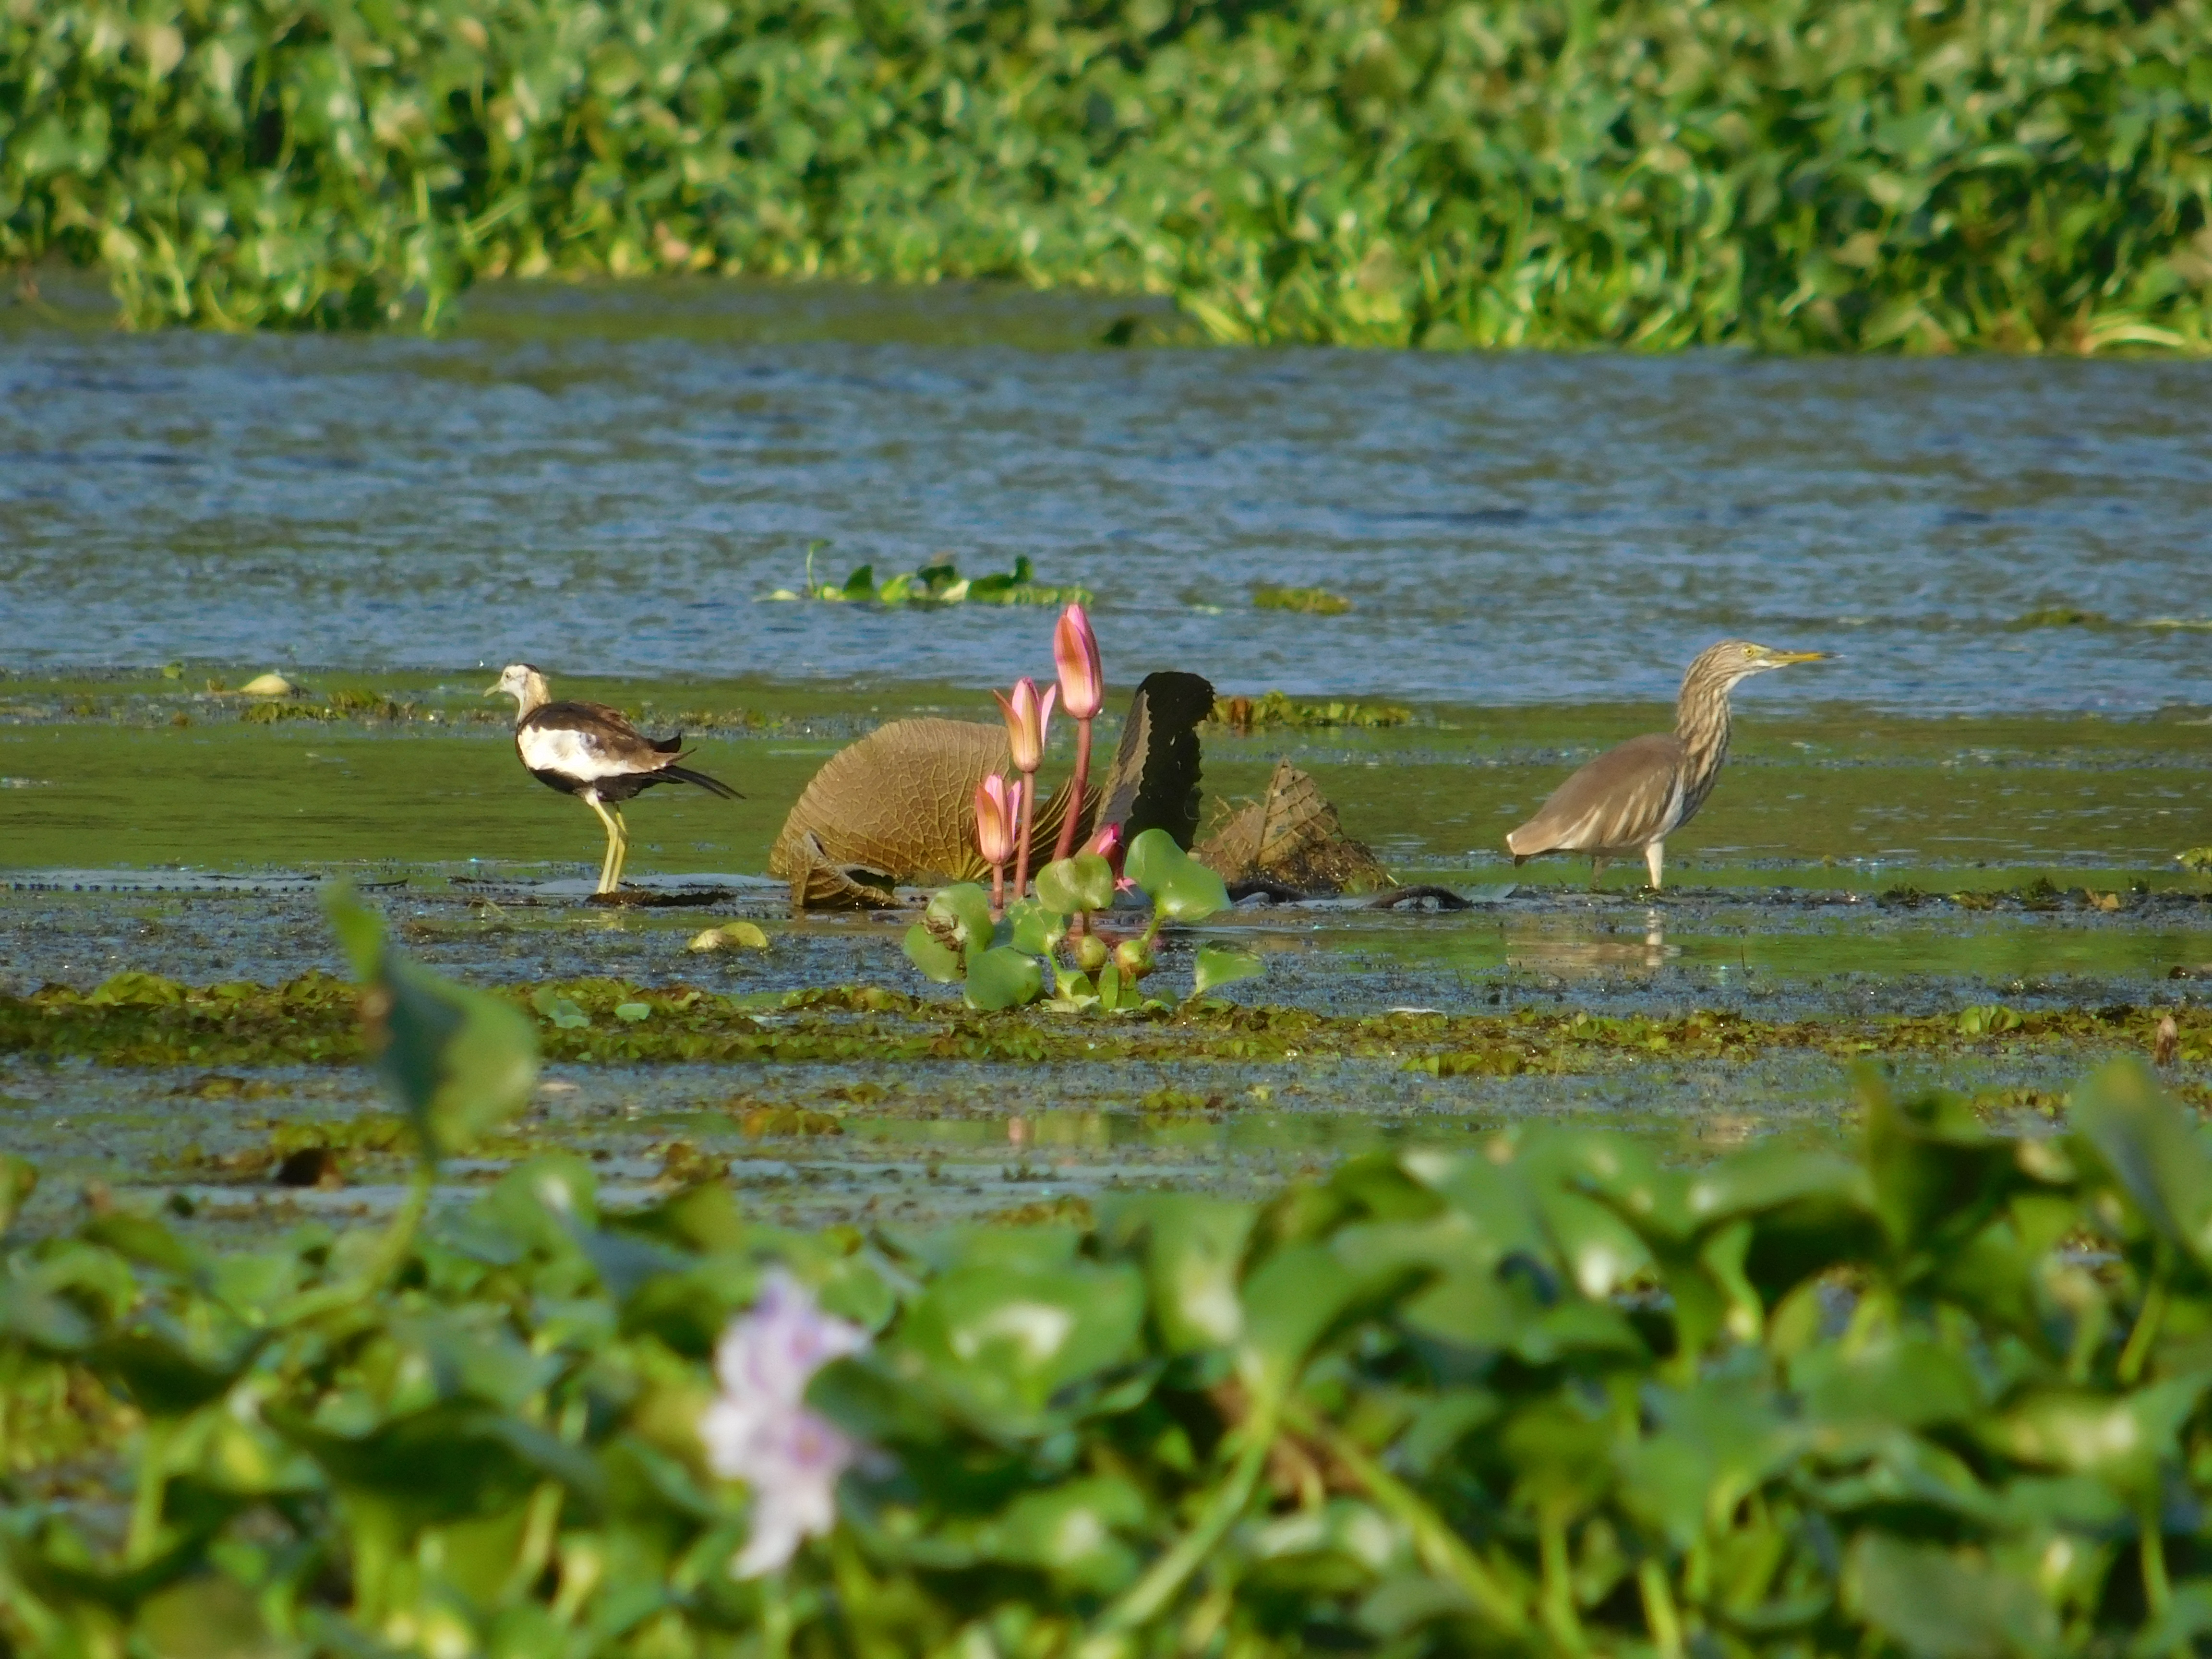
\includegraphics[width=\linewidth]{Figures/scenery.JPG}
    \caption[]{A Pheasant-tailed Jacana and an Indian Pond-Heron at Boat yard.}
    \label{fig:figure-01}
\end{figure}
\item%\
Laniidae%
\begin{enumerate}%
\item%
\begin{description}%
\item[]%
\textit{Lanius cristatus (LC\footnote{National Conservation Status not available. This is Global Conservation Status according to the the National Red List 2021.})}%
\item[]%
\textbf{Brown Shrike}%
\end{description}%
\begin{description}%
\item[H: ]%
Common throughout the island. Can be observed in open country with trees or bushes{[}2{]}.%
\item[D: ]%
The primary diet of this bird includes insects, as well as small birds and mammals.%
\item[R: ]%
Observed in an exact single location located inside the Kaju kele multiple times.%
\end{description}%
\end{enumerate}%
\item%
Laridae%
\begin{enumerate}%
\item%
\begin{description}%
\item[]%
\textit{Chlidonias hybrida (LC\footnote{National Conservation Status not available. This is Global Conservation Status according to the the National Red List 2021.})}%
\item[]%
\textbf{Whiskered Tern}%
\end{description}%
\begin{description}%
\item[H: ]%
Common winter migrant to lowlands but rare in the hills. Marshes, tanks, paddy-fields, coastal lagoons, salt{-}pans, coastal waters, lakes and rivers are the preferred habitats{[}2{]}.%
\item[D: ]%
Small fish, shrimp, and other marine invertebrates. They hunt by dipping their bills into the water while hovering or flying low over the surface.%
\item[R: ]%
Boat yard and the surrounding areas of Bolgoda lake.%
\end{description}%
\item%
\begin{description}%
\item[]%
\textit{Sternula albifrons (VU)}%
\item[]%
\textbf{Little Tern}%
\end{description}%
\begin{description}%
\item[H: ]%
Fairly common and local breeding resident in dry zone and visitor to the wet zone. Can be seen in coastal wetlands and inland tanks{[}2{]}.%
\item[D: ]%
Diet consisting of fish, crustaceans, and invertebrates.%
\item[R: ]%
Boat yard and the surrounding areas of Bolgoda lake. Seen only once%
\end{description}%
\end{enumerate}%
\item%
Leiothrichidae%
\begin{enumerate}%
\item%
\begin{description}%
\item[]%
\textit{Argya affinis (LC)}%
\item[]%
\textbf{Yellow{-}billed Babbler}%
\end{description}%
\begin{description}%
\item[H: ]%
Common breeding resident from lowlands up to mid hills. uncommon and local further in higher hills. Mostly being on the ground can be seen in wooded areas and trees in villages and town gardens. Avoids forests in wet zone and adjoining hills.{[}2{]}.%
\item[D: ]%
Diet includes insects, spiders, small fruits, grains, nectar, and occasionally, lizards or scavenged scraps of food from human habitations.%
\item[R: ]%
Thoughout the university.%
\end{description}%
\end{enumerate}%
\item%
Megalaimidae%
\begin{enumerate}%
\item%
\begin{description}%
\item[]%
\textit{Psilopogon zeylanicus (LC)}%
\item[]%
\textbf{Brown{-}headed Barbet}%
\end{description}%
\begin{description}%
\item[H: ]%
Common breeding resident from lowlands up to mid hills. Uncommon but recorded in higher hills. Forests,open woods.gardens and trees in cultivation are the habitat which can be observed mostly.{[}2{]}.%
\item[D: ]%
Primarily feeds on fruit{-}based diet, consists of wild fruits, berries, and plantation fruits. Also feeds on insects, including ants, termites, and grasshoppers.%
\item[R: ]%
In Kaju kele, Lagaan area and the playground premises.%
\end{description}%
\item%
\begin{description}%
\item[]%
\textit{Psilopogon rubricapillus (LC)}%
\item[]%
\textbf{Sri Lanka Barbet/Crimson{-}fronted Barbet}%
\end{description}%
\begin{description}%
\item[H: ]%
Fairly common endemic locally from wet lowlands up to mid hills. Uncommon but recorded in dry zone. Forests and open wooded country is the preferred habitat{[}2{]}.%
\item[D: ]%
Mainly consists of fruits and insects.%
\item[R: ]%
Observed in Ceremonial courtyard, Kaju Kele and "Thummulla" area.%
\end{description}%
\end{enumerate}%
\item%
Meropidae%
\begin{enumerate}%
\item%
\begin{description}%
\item[]%
\textit{Merops philippinus (CR)}%
\item[]%
\textbf{Blue{-}tailed Bee{-}Eater}%
\end{description}%
\begin{description}%
\item[H: ]%
Fairly common winter migrants throughout the island. Small flocks do breed on eastern dry lowlands. Open areas and the forests are the preferred habitats{[}2{]}.%
\item[D: ]%
Primarily feeds on flying insects, with a particular focus on bees, wasps, butterflies and hornets. %
\item[R: ]%
University ground, around Sumanadasa building, Boat yard, open areas of Kaju Kele. Around the buildings/trees of  ENTC,  Dept. of Civil Engineering and Dept. of Architecture buildings.%
\end{description}%
\end{enumerate}%
\item%
Monarchidae%
\begin{enumerate}%
\item%
\begin{description}%
\item[]%
\textit{Terpsiphone paradisi (LC)}%
\item[]%
\textbf{Asian Paradise{-}Flycatcher/Indian Paradise{-}Flycatcher}%
\end{description}%
\begin{description}%
\item[H: ]%
Two recognised subspecies. One being (T.p.ceylonensis) a fairly common breeding resident found in dry lowlands and adjoining dry lower hills. The other (T.p.paradisi) is a fairly common winter migrant throughout. Open forests, groves and town gardens are the habitat where mostly can be spotted{[}2{]}.%
\item[D: ]%
Feeds mainly on insects.  They usually hunt in the under-story of densely canopied trees.%
\item[R: ]%
Observed in Kaju Kele area and at the boat yard.%
\end{description}%
\end{enumerate}%
\item%
Motacillidae%
\begin{enumerate}%
\item%
\begin{description}%
\item[]%
\textit{Motacilla tschutschensis/flava\footnote{The presence of Eastern Yellow Wagtail in Sri Lanka is still a matter of debate. Hence it could be either of the two species. } (LC\footnote{National Conservation Status not available. This is Global Conservation Status according to the the National Red List 2021.})}%
\item[]%
\textbf{Eastern/Western Yellow Wagtail}%
\end{description}%
\begin{description}%
\item[H: ]%
Common winter migrant to Sri Lanka. Can be observed in damp grasslands and marshes{[}2{]}.%
\item[D: ]%
Primarily feeds on insects, such as midges, flies, beetles, aphids, ants, and various others.%
\item[R: ]%
In the university ground premises.%
\end{description}%
\item%
\begin{description}%
\item[]%
\textit{Dendronanthus indicus (LC\footnote{National Conservation Status not available. This is Global Conservation Status according to the the National Red List 2021.})}%
\item[]%
\textbf{Forest Wagtail}%
\end{description}%
\begin{description}%
\item[H: ]%
Fairly common winter migrant throughout. Paths and open spaces in wooded areas are the preferred habitat
{[}2{]}.%
\item[D: ]%
The diet primarily includes tiny invertebrates like ants, beetles and various other insects. It also includes spiders, small mollusks, and worms.%
\item[R: ]%
Observed multiple times but only at hotspot 2, Kaju kele.%
\end{description}%
\item%
\begin{description}%
\item[]%
\textit{Anthus rufulus (LC)}%
\item[]%
\textbf{Paddyfield Pipit}%
\end{description}%
\begin{description}%
\item[H: ]%
Fairly common breeding resident throughout the country. Grasslands and low scrub are the preferred habitat{[}2{]}.%
\item[D: ]%
Primary diet consists of small insects, yet it also indulges in larger prey such as beetles, small snails, and worms while traversing the ground. %
\item[R: ]%
In university ground premises.%
\end{description}%
\end{enumerate}%
\item%
Muscicapidae%
\begin{enumerate}%
\item%
\begin{description}%
\item[]%
\textit{Copsychus saularis (LC)}%
\item[]%
\textbf{Oriental Magpie{-}Robin}%
\end{description}%
\begin{description}%
\item[H: ]%
Common breeding resident throughout Sri Lanka. Gardens, scrub, open forest and cultivation are the preferred habitats while avoiding interior of wet forests{[}2{]}.%
\item[D: ]%
Primary diet comprises insects and other invertebrates. Occasion, they may also consume flower nectar, geckos, leeches and centipedes.%
\item[R: ]%
Around the Faculty of IT, Kaju kele and boat yard.%
\end{description}%
\item%
\begin{description}%
\item[]%
\textit{Muscicapa muttui (LC\footnote{National Conservation Status not available. This is Global Conservation Status according to the the National Red List 2021.})}%
\item[]%
\textbf{Brown{-}breasted Flycatcher}%
\end{description}%
\begin{description}%
\item[H: ]%
Uncommon winter migrant to wet lowlands and up to lower hills. local and less common in mid hills and dry lowlands. Forest, well wooded areas often near streams are the places to spot easily{[}2{]}.%
\item[D: ]%
Primarily feed on insects. Their common food items include beetles, caterpillars, flies, and spiders.%
\item[R: ]%
Observed around the Jack trees located near the library%
\end{description}%
\item%
\begin{description}%
\item[]%
\textit{Saxicoloides fulicatus (LC)}%
\item[]%
\textbf{Indian Robin}%
\end{description}%
\begin{description}%
\item[H: ]%
Common breeding resident in dry lowlands, rare and local in wet lowlands up to midhills. Forest, open scrub, cultivation edges and the gardens are the habitats that mostly can be observed{[}2{]}.%
\item[D: ]%
Primary diet consists of insects, although they are also known to consume frogs and lizards, particularly when feeding their young at the nest.%
\item[R: ]%
Observed only once in the courtyard of the Dept. Of Chemical Engineering%
\end{description}%
\item%
\begin{description}%
\item[]%
\textit{Muscicapa dauurica (LC\footnote{National Conservation Status not available. This is Global Conservation Status according to the the National Red List 2021.})}%
\item[]%
\textbf{Asian Brown Flycatcher}%
\end{description}%
\begin{description}%
\item[H: ]%
Fairly common winter migrant in lowlands up to mid hills. Open wooded areas, plantations and garden are the preferred habitat{[}2{]}.%
\item[D: ]%
Predominantly feeds on flying insects, employing a sallying technique where it launches from a perch to catch its prey in mid{-}air.%
\item[R: ]%
Open area behind the Boat yard and inside Kaju kele.%
\end{description}%
\end{enumerate}%
\item%
Nectariniidae%
\begin{enumerate}%
\item%
\begin{description}%
\item[]%
\textit{Leptocoma zeylonica (LC)}%
\item[]%
\textbf{Purple{-}rumped Sunbird}%
\end{description}%
\begin{description}%
\item[H: ]%
Common breeding resident in lowlands and up to mid hills. Rare in areas above that. Cultivation, gardens and forest are the places for look for.{[}2{]}.%
\item[D: ]%
Primarily feeds on nectar, occasionally supplementing their diet with insects, especially when tending to their young.%
\item[R: ]%
In Kaju Kele area, trees around the Bhavana and trees of Ceremonial courtyard. %
\end{description}%
\item%
\begin{description}%
\item[]%
\textit{Cinnyris lotenius (LC)}%
\item[]%
\textbf{Long{-}billed Sunbird/Loten's Sunbird}%
\end{description}%
\begin{description}%
\item[H: ]%
Fairly common breeding resident throughout Sri Lanka. But less common in the high hills. Can be observed in forests, wooded areas and gardens{[}2{]}.%
\item[D: ]%
Consumes small insects and spiders, similar to other Sunbird species.%
\item[R: ]%
Surrounding area of Dept. of FD \& PD. In the trees around the Bhavana and trees of Ceremonial courtyard.%
\end{description}%
\end{enumerate}%
\item%
Oriolidae%
\begin{enumerate}%
\item%
\begin{description}%
\item[]%
\textit{Oriolus kundoo (LC\footnote{National Conservation Status not available. This is Global Conservation Status according to the the National Red List 2021.})}%
\item[]%
\textbf{Indian Golden Oriole}%
\end{description}%
\begin{description}%
\item[H: ]%
Rare winter migrant to lowlands and lower hills. Solitary and can be seen in wooded areas{[}2{]}.%
\item[D: ]%
Feeds mainly of wild fruits and on insects. %
\item[R: ]%
Observed only once in the wooded area behind the main library building%
\end{description}%
\item%
\begin{description}%
\item[]%
\textit{Oriolus xanthornus (LC)}%
\item[]%
\textbf{Black{-}hooded Oriole}%
\end{description}%
\begin{description}%
\item[H: ]%
Fairly common breeding resident found in lowlands up to mid hills. Forests, wooded areas and trees in villages and town gardens are the habitats where can be easily seen{[}2{]}.%
\item[D: ]%
Diet ranges from insects like caterpillars and beetles to fruits and nectar, positions them as important contributors to their ecosystem.%
\item[R: ]%
Throughout the university.%
\end{description}%
\end{enumerate}%
\item%
Pelecanidae%
\begin{enumerate}%
\item%
\begin{description}%
\item[]%
\textit{Pelecanus philippensis (LC)}%
\item[]%
\textbf{Spot{-}billed Pelican}%
\end{description}%
\begin{description}%
\item[H: ]%
Common breeding resident throughout the dry lowlands. Introduced population commonly can be observed in the wet zone.  Can be commonly observed in tanks, lakes, lagoons and marshlands{[}2{]}.%
\item[D: ]%
Primarily fish, including introduced species like catfish, carp, and tilapia and consume frogs, crustaceans, and even small birds occasionally.%
\item[R: ]%
Boat yard and the surrounding areas of Bolgoda lake. Mostly observed in flight.%
\end{description}%
\end{enumerate}%
\item%
Phalacrocoracidae%
\begin{enumerate}%
\item%
\begin{description}%
\item[]%
\textit{Phalacrocorax fuscicollis (LC)}%
\item[]%
\textbf{Indian Cormorant}%
\end{description}%
\begin{description}%
\item[H: ]%
Very common breeding resident in dry lowlands. Less commonly observed in wet lowlands and lower hills too. Marshlands, tanks, lakes, rivers and lagoons are the preferred habitat{[}2{]}.%
\item[D: ]%
Primarily fish, but also consumes crustaceans, mollusks, and aquatic insects.%
\item[R: ]%
Boat yard and the surrounding areas of Bolgoda lake.%
\end{description}%
\item%
\begin{description}%
\item[]%
\textit{Phalacrocorax carbo (NT)}%
\item[]%
\textbf{Great Cormorant}%
\end{description}%
\begin{description}%
\item[H: ]%
Uncommon breeding resident in dry lowlands and rarely seen in wet lowlands. Could be spotted in larger tanks and coastal lagoons{[}2{]}.%
\item[D: ]%
Primarily fish, especially eel species and catfish. They also hunt frogs, crabs, and other aquatic animals.%
\item[R: ]%
Boat yard and the surrounding areas of Bolgoda lake.%
\end{description}%
\item%
\begin{description}%
\item[]%
\textit{Microcarbo niger (LC)}%
\item[]%
\textbf{Little Cormorant}%
\end{description}%
\begin{description}%
\item[H: ]%
Very common breeding resident mainly from lowlands to lower hills. Present in higher hills but less common. Lakes, tanks, marshes, paddy-fields, rivers, streams and lagoons are preferred habitats{[}2{]}.%
\item[D: ]%
Primarily consume fish, occasionally on crustaceans and amphibians. They engage in diving to capture their prey and resurface to swallow it.%
\item[R: ]%
Boat yard and the surrounding areas of Bolgoda lake.%
\end{description}%
\end{enumerate}%
\item%
Picidae%
\begin{enumerate}%
\item%
\begin{description}%
\item[]%
\textit{Dinopium psarodes (LC)}%
\item[]%
\textbf{Red{-}backed Flameback}%
\end{description}%
\begin{description}%
\item[H: ]%
Fairly common breeding resident in the southern part of the country. Forests, coconut plantations and trees in open country are the areas where can be easily observed{[}2{]}.%
\item[D: ]%
Primary diet consists of larvae and pupae of ants. Consumes invertebrates such as spiders, caterpillars, weevils, and beetles.%
\item[R: ]%
Kaju kele,Boat yard, wooded areas around the steel building, and Lagaan.%
\end{description}%
\end{enumerate}%
\item%
Psittacidae%
\begin{enumerate}%
\item%
\begin{description}%
\item[]%
\textit{Loriculus beryllinus (LC)}%
\item[]%
\textbf{Sri Lanka Hanging{-}Parrot}%
\end{description}%
\begin{description}%
\item[H: ]%
Endemic and fairly common bird found in wet lowlands to mid hills. Restricted to the foothill areas in the dry lowlands. Can be mostly seen in forests and wooded areas{[}2{]}.%
\item[D: ]%
Their natural diet consists mainly of fruits; particularly wild figs, guava and berries, as well as flower buds and blossoms. Also feeds on nectar and seeds.%
\item[R: ]%
Surrounding areas of university playground and Ceremonial courtyard.%
\end{description}%
\item%
\begin{description}%
\item[]%
\textit{Psittacula krameri (LC)}%
\item[]%
\textbf{Rose{-}ringed Parakeet}%
\end{description}%
\begin{description}%
\item[H: ]%
Common breeding resident from lowlands to mid hills and a small population recorded in higher hills. Forests and wooded areas by villages and towns are the preferred habitat. Can be observed even in densely populated areas as well{[}2{]}.%
\item[D: ]%
Usually feed on buds, fruits, vegetables, nuts, berries, and seeds.%
\item[R: ]%
In flight at evenings/mornings above the university ground premises. Very common inside Kaju kele.%
\end{description}%
\end{enumerate}%
\item%
Pycnonotidae%
\begin{enumerate}%
\item%
\begin{description}%
\item[]%
\textit{Pycnonotus cafer (LC)}%
\item[]%
\textbf{Red{-}vented Bulbul}%
\end{description}%
\begin{description}%
\item[H: ]%
Very common breeding resident that can be seen all around the country. Easy to spot in forest fringe, open forest, cultivated lands and trees in habitation.  Avoid interior of thick forests in wet zone{[}2{]}.%
\item[D: ]%
Diet encompasses a variety of food sources, including fruits, flower petals, nectar, and insects. Occasionally consume house geckos.%
\item[R: ]%
Throughout the university.%
\end{description}%
\item%
\begin{description}%
\item[]%
\textit{Pycnonotus luteolus (LC)}%
\item[]%
\textbf{White{-}browed Bulbul}%
\end{description}%
\begin{description}%
\item[H: ]%
Common breeding resident mainly in dry lowlands. Uncommon in wet lowlands and up to mid hills. Dry forests, scrub and gardens are the preferred habitat{[}2{]}.%
\item[D: ]%
Primarily feed on a diet consisting of fruit, nectar, and insects.%
\item[R: ]%
In kaju Kele and around the trees near Steel building%
\end{description}%
\end{enumerate}%
\item%
Rallidae%
\begin{enumerate}%
\item%
\begin{description}%
\item[]%
\textit{Amaurornis phoenicurus (LC)}%
\item[]%
\textbf{White{-}breasted Waterhen}%
\end{description}%
\begin{description}%
\item[H: ]%
Common breeding resident throughout the Island. Marshes, paddy fields and any other wet areas with thick cover are the preferred habitat{[}2{]}.%
\item[D: ]%
Aquatic plants, seeds, fruits, insects, and small fish. They forage by wading in shallow water and picking food from the surface.%
\item[R: ]%
Boat yard and the surrounding shallow areas of Bolgoda lake.%
\end{description}%
\item%
\begin{description}%
\item[]%
\textit{Porphyrio poliocephalus (LC)}%
\item[]%
\textbf{Gray{-}headed Swamphen/Purple Swamphen}%
\end{description}%
\begin{description}%
\item[H: ]%
Locally common breeding resident in the lowlands. Reed beds, marshes, paddy-fields and weedy tanks are the habitat types which can be easily spotted{[}2{]}.%
\item[D: ]%
Omnivorous, feeding on insects, worms, frogs, small fish, seeds, fruits, and leaves.%
\item[R: ]%
Boat yard and the surrounding shallow areas of Bolgoda lake%
\end{description}%
\end{enumerate}%
\item%
Recurvirostridae%
\begin{enumerate}%
\item%
\begin{description}%
\item[]%
\textit{Himantopus himantopus (LC)}%
\item[]%
\textbf{Black{-}winged Stilt}%
\end{description}%
\begin{description}%
\item[H: ]%
Fairly common breeding resident in dry lowlands. A few birds breed in wet lowlands while others are winter migrants in the lowlands. Freshwater and brackish shallow waters in marshes, lagoons and tanks are the preferred habitats{[}2{]}.%
\item[D: ]%
Uses the sharp bills to peck and ingest only very small food such as molluscs, crustaceans, algae, flies and aquatic insects.%
\item[R: ]%
Observed at Boat yard only once as a flock in flight.%
\end{description}%
\end{enumerate}%
\item%
Strigidae%
\begin{enumerate}%
\item%
\begin{description}%
\item[]%
\textit{Ninox scutulata (NT)}%
\item[]%
\textbf{Brown Hawk{-}Owl/Brown Boobook}%
\end{description}%
\begin{description}%
\item[H: ]%
A common breeding resident. Can be found throughout the island except in the higher hills. Can be observed in forests and other well wooded areas of villages and towns.{[}2{]}.%
\item[D: ]%
Primary diet includes insects, encompassing large insects as well as small mammals, birds, frogs, and lizards.%
\item[R: ]%
Around Lagaan and Faculty of IT at night.%
\end{description}%
\item%
\begin{description}%
\item[]%
\textit{Otus bakkamoena (LC)}%
\item[]%
\textbf{Indian Scops{-}Owl/Collared Scops{-}Owl}%
\end{description}%
\begin{description}%
\item[H: ]%
Fairly common breeding resident found throughout the island. Uncommon in the higher hills. Avoid interior of wet evergreen forests and typically found inside well wooded areas and residential gardens of villages and towns{[}2{]}.%
\item[D: ]%
Primary diet comprises insects, including beetles and grasshoppers. May also prey on small vertebrates such as rodents, small birds, and lizards.%
\item[R: ]%
In seetha gangula area at night. One specimen was recorded inside a building during day time.%
\end{description}%
\end{enumerate}%
\item%
Sturnidae%
\begin{enumerate}%
\item%
\begin{description}%
\item[]%
\textit{Acridotheres tristis (LC)}%
\item[]%
\textbf{Common Myna}%
\end{description}%
\begin{description}%
\item[H: ]%
Common breeding throughout. Forest edges, trees in open areas, village and town gardens are the places to look for.{[}2{]}.%
\item[D: ]%
Diet includes insects, arachnids, crustaceans, reptiles, small mammals, seeds, grains, fruits, and discarded waste from human habitation.%
\item[R: ]%
Throughout the university premises.%
\end{description}%
\end{enumerate}%
\item%
Threskiornithidae%
\begin{enumerate}%
\item%
\begin{description}%
\item[]%
\textit{Threskiornis melanocephalus (LC)}%
\item[]%
\textbf{Black{-}headed Ibis}%
\end{description}%
\begin{description}%
\item[H: ]%
Common breeding resident in lowlands. Regularly observed near freshwater tanks, marshes and paddy-fields{[}2{]}.%
\item[D: ]%
Insects, worms, snails, and small frogs. They forage in wetlands, rice paddies, and fields, probing the ground with their long bills.%
\item[R: ]%
Boat yard and the surrounding areas of Bolgoda lake.%
\end{description}%
\end{enumerate}%
\item%
Zosteropidae%
\begin{enumerate}%
\item%
\begin{description}%
\item[]%
\textit{Zosterops palpebrosus (LC)}%
\item[]%
\textbf{Indian White{-}Eye/Oriental White{-}Eye}%
\end{description}%
\begin{description}%
\item[H: ]%
Fairly common breeding resident from lowlands up to mid hills. Uncommon in high hills. Can be seen around trees{[}2{]}.%
\item[D: ]%
While primarily insectivorous, it also incorporates nectar and various fruits into its diet.%
\item[R: ]%
Tree tops behind the boat yard at the area where the Kaju kele starts.%
\end{description}%
\end{enumerate}%
\end{itemize}
